\documentclass[10pt, a4j, dvipdfmx]{jarticle}
\usepackage{titlesec}
\usepackage[dvipdfmx]{graphicx}
\usepackage[dvipdfmx]{color}
\usepackage{float}
\usepackage{wrapfig}
\usepackage{subfigure}
\usepackage{caption}
\usepackage{multirow}
\usepackage{amsmath}
\usepackage{amssymb}

\graphicspath{{../image/}}

\makeatletter
\newcommand{\figcaption}[1]{\def\@captype{figure}\caption{#1}}
\newcommand{\tblcaption}[1]{\def\@captype{table}\caption{#1}}
\makeatother

\def\para{%
\setlength{\unitlength}{1pt}%
\thinlines %
\begin{picture}(12, 12)%
\put(0,0){/}
\put(2,0){/}
\end{picture}%
}%

\title{トランジスタ増幅}
\author{4年 電子システム工学科 40番  山地 駿徹}


\begin{document}
    \section{原理}
    \subsection*{発信条件}
    周波数fで入力$I_i$と出力$I_o$が同相であり,$I_o = A \cdot I_i$,$A > 1$となる増幅器を考える.
    図\ref{fig:1}のように,出力を入力に接続すると,外部から信号を入れなくても,振幅の小さな振動から大きな振動へと成長し,信号は消滅しない.

    このことから,発信可能の条件は,$R(A) > 1$,$G(A) = 0$となり,これを発信可能条件という.

    発信が定常的になったときは,$R(A') = 1$,$G(A') =0$となり,これを発信持続条件と呼ぶ,
    このときの$A'$は$A$とは異なる.

    \subsection*{CR位相型発振回路の解析}
    \begin{figure}[H]
        \centering
        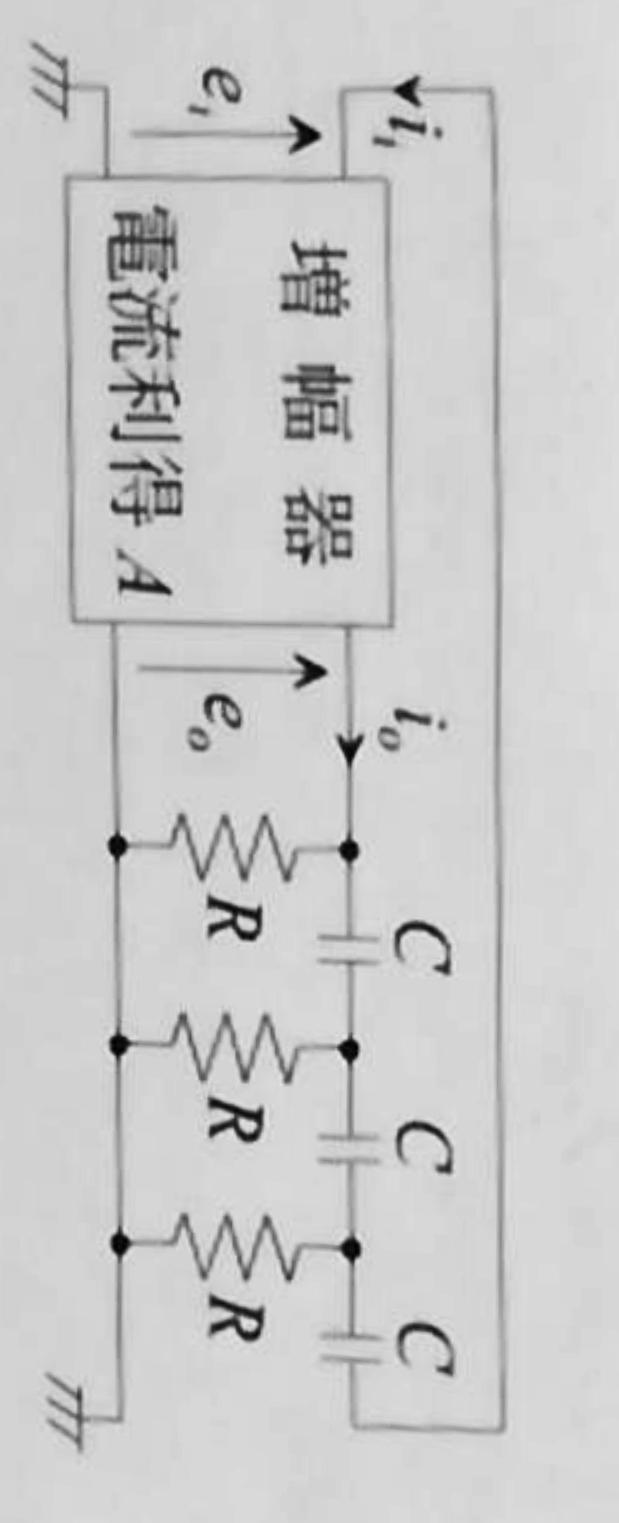
\includegraphics[width=50mm, angle=90]{txt-1.jpg}
        \figcaption{移相型発振回路(進相形,トランジスタ)}
        \label{fig:txt-1}
    \end{figure}
    位相素子図に対するF-パラメータは,\\
    \begin{equation*}
        \begin{bmatrix}
            e_1 \\
            i_1 \\
        \end{bmatrix}
        =
        \begin{bmatrix}
            A & B \\
            C & D \\
        \end{bmatrix}
        \begin{bmatrix}
            e_2 \\
            i_2 \\
        \end{bmatrix}
    \end{equation*}
    \\として\\
    \begin{eqnarray*}
        \begin{array}{rr}
            A = 1,& B = \frac{1}{j\omega C} \\
            C = \frac{1}{R},& D = 1 + \frac{1}{j\omega CR} \\      
        \end{array}
    \end{eqnarray*}
    \\で与えられる.
    ここで,$k = 1/\omega CR$とおけば,3段の位相素子に対するF-パラメータは\\
    \begin{equation*}
        \begin{bmatrix}
            e_1 \\
            i_1 \\
        \end{bmatrix}
        =
        \begin{bmatrix}
            A & B \\
            C & D \\
        \end{bmatrix}
        \begin{bmatrix}
            e_2 \\
            i_2 \\
        \end{bmatrix}
    \end{equation*}
    \\より,\\
    \begin{eqnarray*}
        \begin{bmatrix}
            A & B \\
            C & D \\
        \end{bmatrix}^3
        & = &
        \begin{bmatrix}
            A^3 + ABC + BCD & A^2B + B^2 + ABD + BD^2 \\
            A^2C + ADC + C^2B + CD^2 & ABC + 2BCD + D^3 \\
        \end{bmatrix}\\
        & = &
        \begin{bmatrix}
            (1 - k^2) - j3k & -R\{4k^2 + jk(3 - k^2)\} \\
            \frac{1}{R}\{(3-k^2)-j4k\} & (1-5k^2)-jk(6-k^2) \\
        \end{bmatrix}
    \end{eqnarray*}
    となる.
    トランジスタの入力インピーダンス$r_ie$が$r_ie<<R$で$r_ie\simeq0$と考えれば,$e_1=0$となる.
    \begin{eqnarray*}
        e_0 = \{(1-k^2) - j3k\}e_1 - R\{(1-k^2) + jk(3-k^2)\}i_1 \\
        i_0 = \frac{1}{R}\{(3-k^2) - j4k\}e_1 - \{(1-5k^2) - jk(6-k^2)\}i_1\\
    \end{eqnarray*}
    において,$e_1=0$を用いると,上式の第2式は,
    \begin{equation*}
        i_0 = \{(1-5k^2) - jk(6-k^2)\}i_i
    \end{equation*}
    となる.$i_0/i_i$は増幅器の電流利得となり,$i_0/i_i$が同装花逆走であれば,上式の虚数部はゼロとなるから,
    \begin{equation*}
        k^2 = 6
    \end{equation*}
    すなわち
    \begin{equation*}
        \omega^2 = 1/6C^2R^2
    \end{equation*}
    となり
    \begin{equation*}
        i_0/i_i = -29
    \end{equation*}
    となる.発信条件は,増幅器の入出力電流位相は逆相で
    \begin{eqnarray*}
        f = \frac{1}{2\pi\sqrt{6}CR} & 周波数条件 \\
        |A| \geq 29 & 電流振幅条件 \\
    \end{eqnarray*}
    が得られる.

    \section{実験方法}
    \subsection*{CR移相型発振回路の設計・制作}
    \begin{enumerate}
        \item トランジスタの静特性を求める.($I_C$-$V_{CE}$特性,$I_B$-$V_{BE}$特性)
        \item 前述の周波数条件より発振周波数を求める.
        \item 発信振幅を決める.(コレクタ側で振幅を$e_m$とする)
        \item 交流負荷$Z_{AC} \simeq B/D$を求める.(前述の周波数条件より$k = 6$なので$|Z_{AC}| \simeq 0.87R$)
        \item 動作点$Q$を交流負荷に対して直線部分の中央に決める.\\
              $V_{CEQ} \simeq e_m$,$I_{CQ} \simeq e_m/|Z_{AC}|$
        \item 静特性曲線より$V_{BEQ}$,$I_{BQ}$を求める.
        \item 電源電圧を決める.$IC 74HC00の端子接続図R_E$が決まる.
        \item 安定度(または,$f = I_2/I_{BQ}$)を決めて,$R_{B1}$,$R_{B2}$を求める.
    \end{enumerate}
    (注) 実際には,前回制作したぞ副回路の$R_C$の代わりに移相回路を接続し,移相回路の出力を増幅回路の入力に接続すればよい.[~$\because |Z_{AC}| \simeq 0.87R$より]
    
    したがって,$R = R_C$とし,周波数条件より$C$を求める.前回の増幅回路をそのまま利用し,移相回路の$CR$を新たに配線すれば良い.

    \subsection*{CR移相回路のボード線図の測定}
    発振回路を制作する前に,求めた$C$と$R$を用いて図のような移相回路の入出力の振幅と移相の関係を測定する.発振器は既製の低周波発振器を用い,$R_i$は$100\Omega$〜数$100\Omega$とする.
    測定すべきは電流の波形の位相差であるが,実際に測定する(できる)位相は,電圧波形である.
    従って,$C_3$の電圧降下$e_O$と$I_O$の位相差($\pi/2$)を考慮して補正しなければならない.
    \begin{figure}[H]
        \begin{minipage}{0.5\hsize}
          \centering
          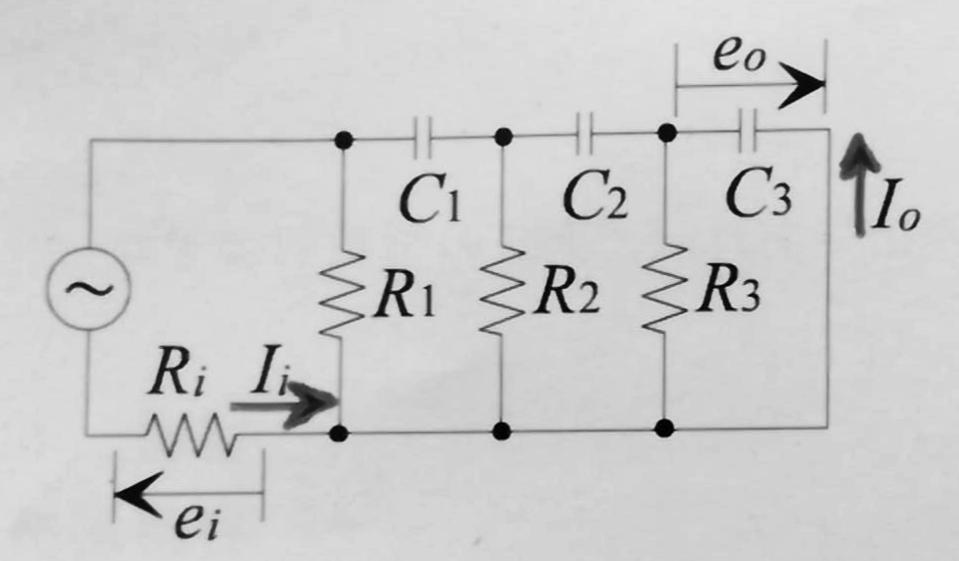
\includegraphics[height=40mm]{txt-2.jpg}
          \caption{移相回路}
        \end{minipage}
        \begin{minipage}{0.5\hsize}
          \centering
          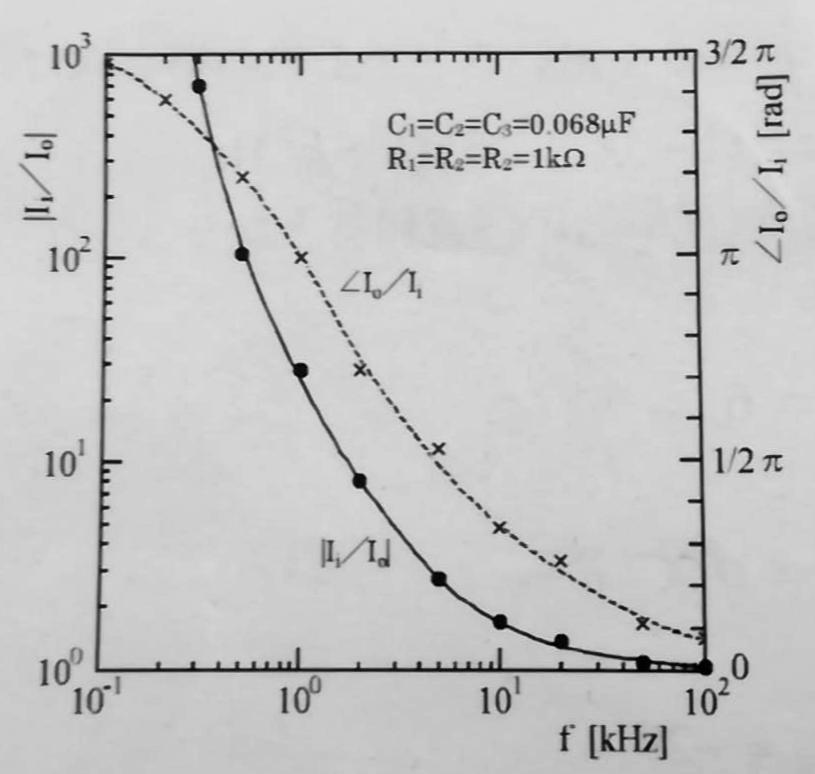
\includegraphics[height=40mm]{txt-3.jpg}
          \caption{ボード線図}
        \end{minipage}
    \end{figure}
    また,$e_i$と$e_O$を2現象オシロで測定する場合,プローブのアースを共通にしなければならないので,$e_O$は実際に測定するのは$-e_O$を測定することになり,位相は反転している(位相差:$\pi$)ことを考慮して補正しなければならない.すなわち,
    \begin{figure}[H]
        \begin{minipage}{0.5\hsize}
            \begin{equation*}
                \angle \frac{-e_O}{e_i} = \theta
            \end{equation*}
        \end{minipage}
        \begin{minipage}{0.5\hsize}
            \begin{equation*}
                \angle \frac{i_O}{i_i} = \theta + \frac{\pi}{2} - \pi = \theta - \frac{\pi}{2}
            \end{equation*}
        \end{minipage}
      \end{figure}

      \subsection*{CR移相型発振回路の制作}
      増幅回路に移相回路のCRを新たに配線してCR移相型発振回路を制作し,発振を確認する.
      波形が歪んでいるときは,$R_b'$($100\Omega$〜数$100\Omega$)を接続して波形の変化を見る.
      \begin{figure}[H]
        \begin{minipage}{0.5\hsize}
          \centering
          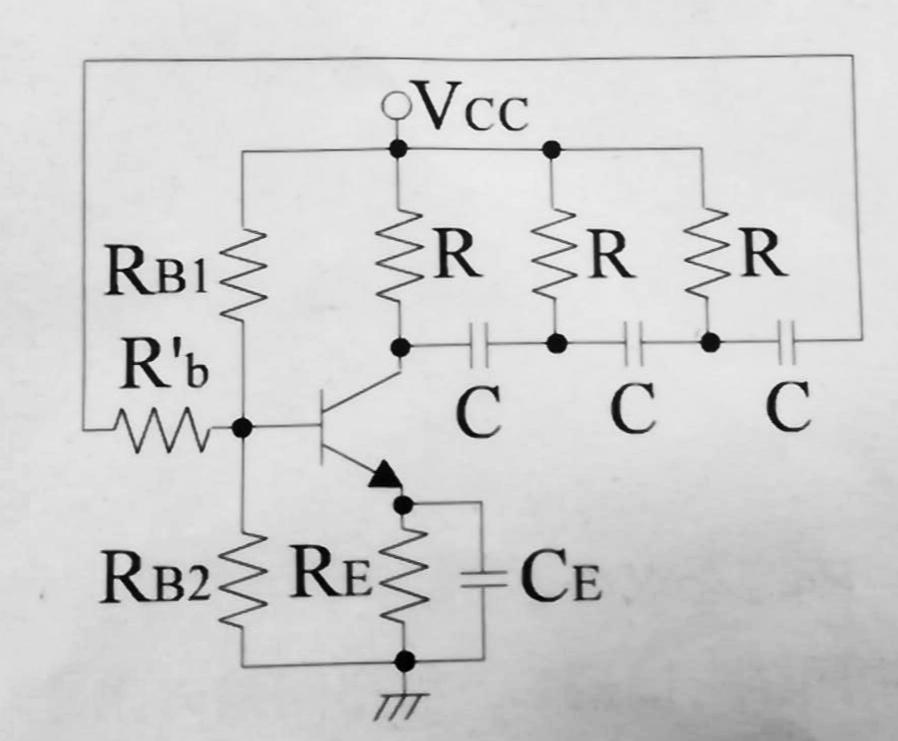
\includegraphics[height=40mm]{txt-4.jpg}
          \caption{発振回路}
        \end{minipage}
        \begin{minipage}{0.5\hsize}
          \centering
          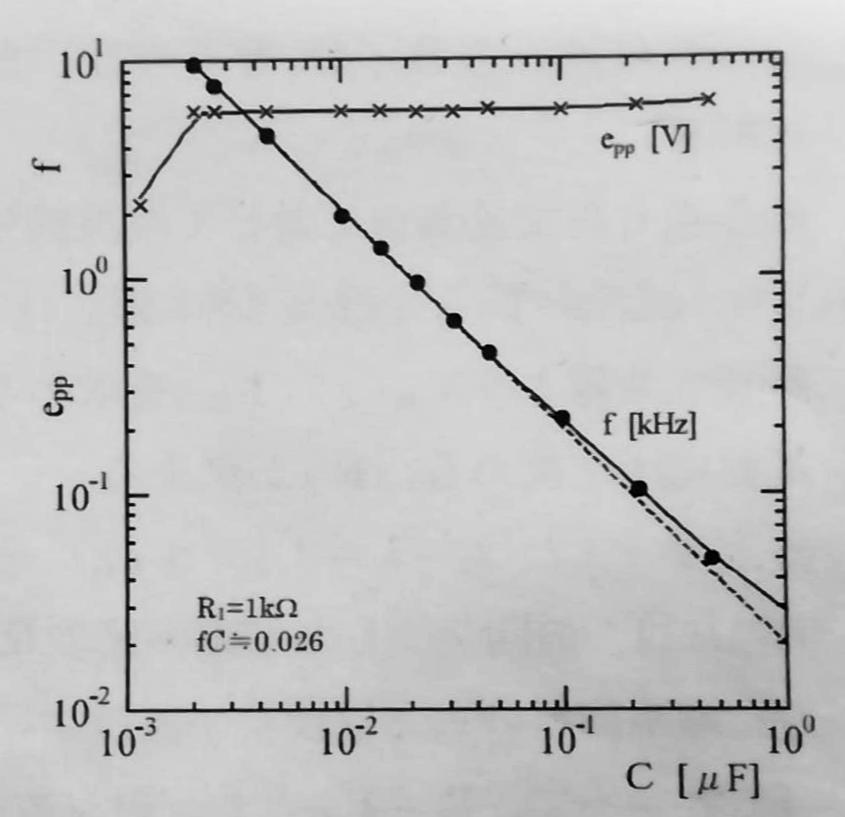
\includegraphics[height=40mm]{txt-5.jpg}
          \caption{容量-周波数特性}
        \end{minipage}
      \end{figure}

      \subsection*{移相器の容量-周波数特性の測定}
      制作したCR移相型発振回路の移相器の容量Cを変えて発振周波数の変化および発振振幅の peak to peak 値の変化を測定する.

      \section{結果の処理}
      2.実験方法 に示した手順に従って実験を行った.
      \subsection{CR移相型発振回路の設計・制作}
      \begin{enumerate}
        \item トランジスタの静特性を求める.($I_C$-$V_{CE}$特性,$I_B$-$V_{BE}$特性)\\
                前回の実験で測定した,トランジスタの静特性を使用する.以下に特性図を示す.
                \begin{figure}[H]
                    \begin{minipage}{0.5\hsize}
                      \centering
                      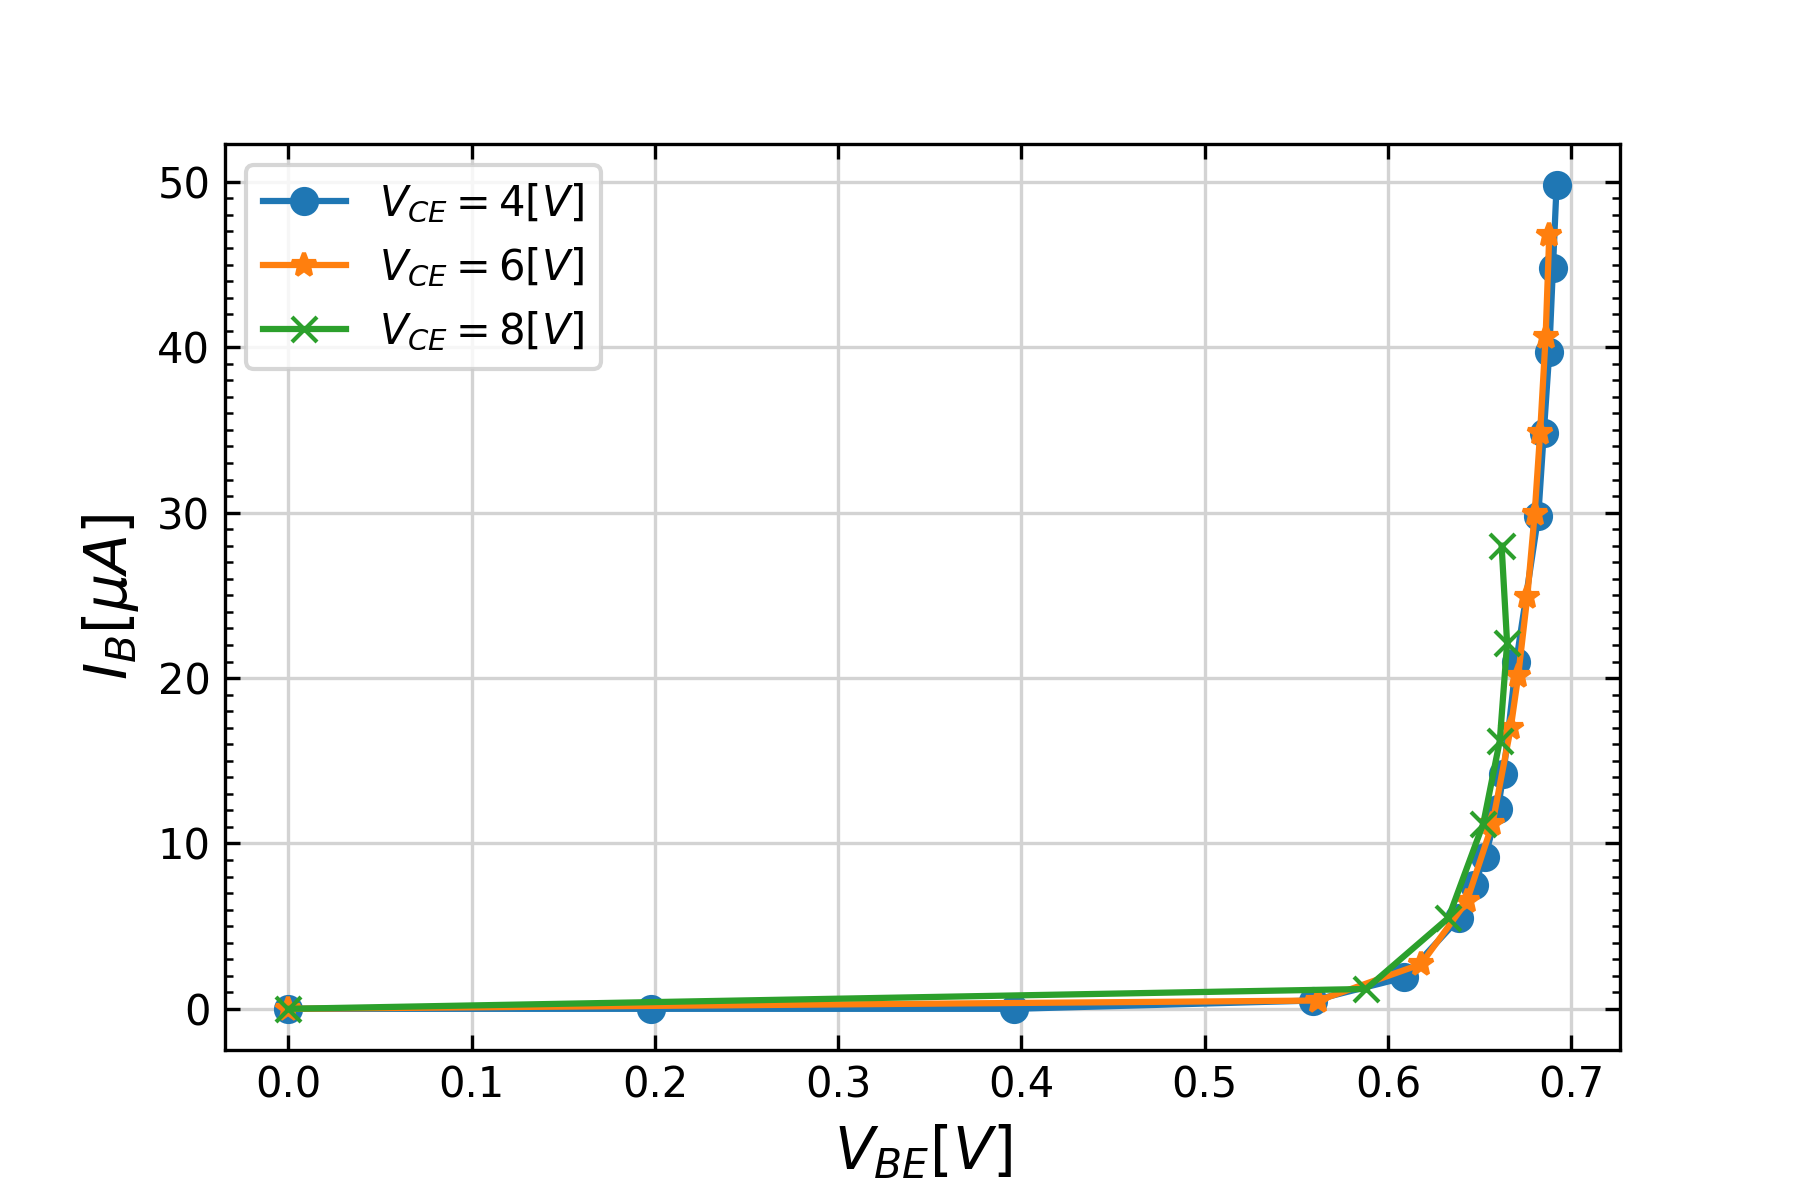
\includegraphics[width=75mm]{Ic-Vce.png}
                      \caption{$I_C$-$V_{CE}$特性}
                    \end{minipage}
                    \begin{minipage}{0.5\hsize}
                      \centering
                      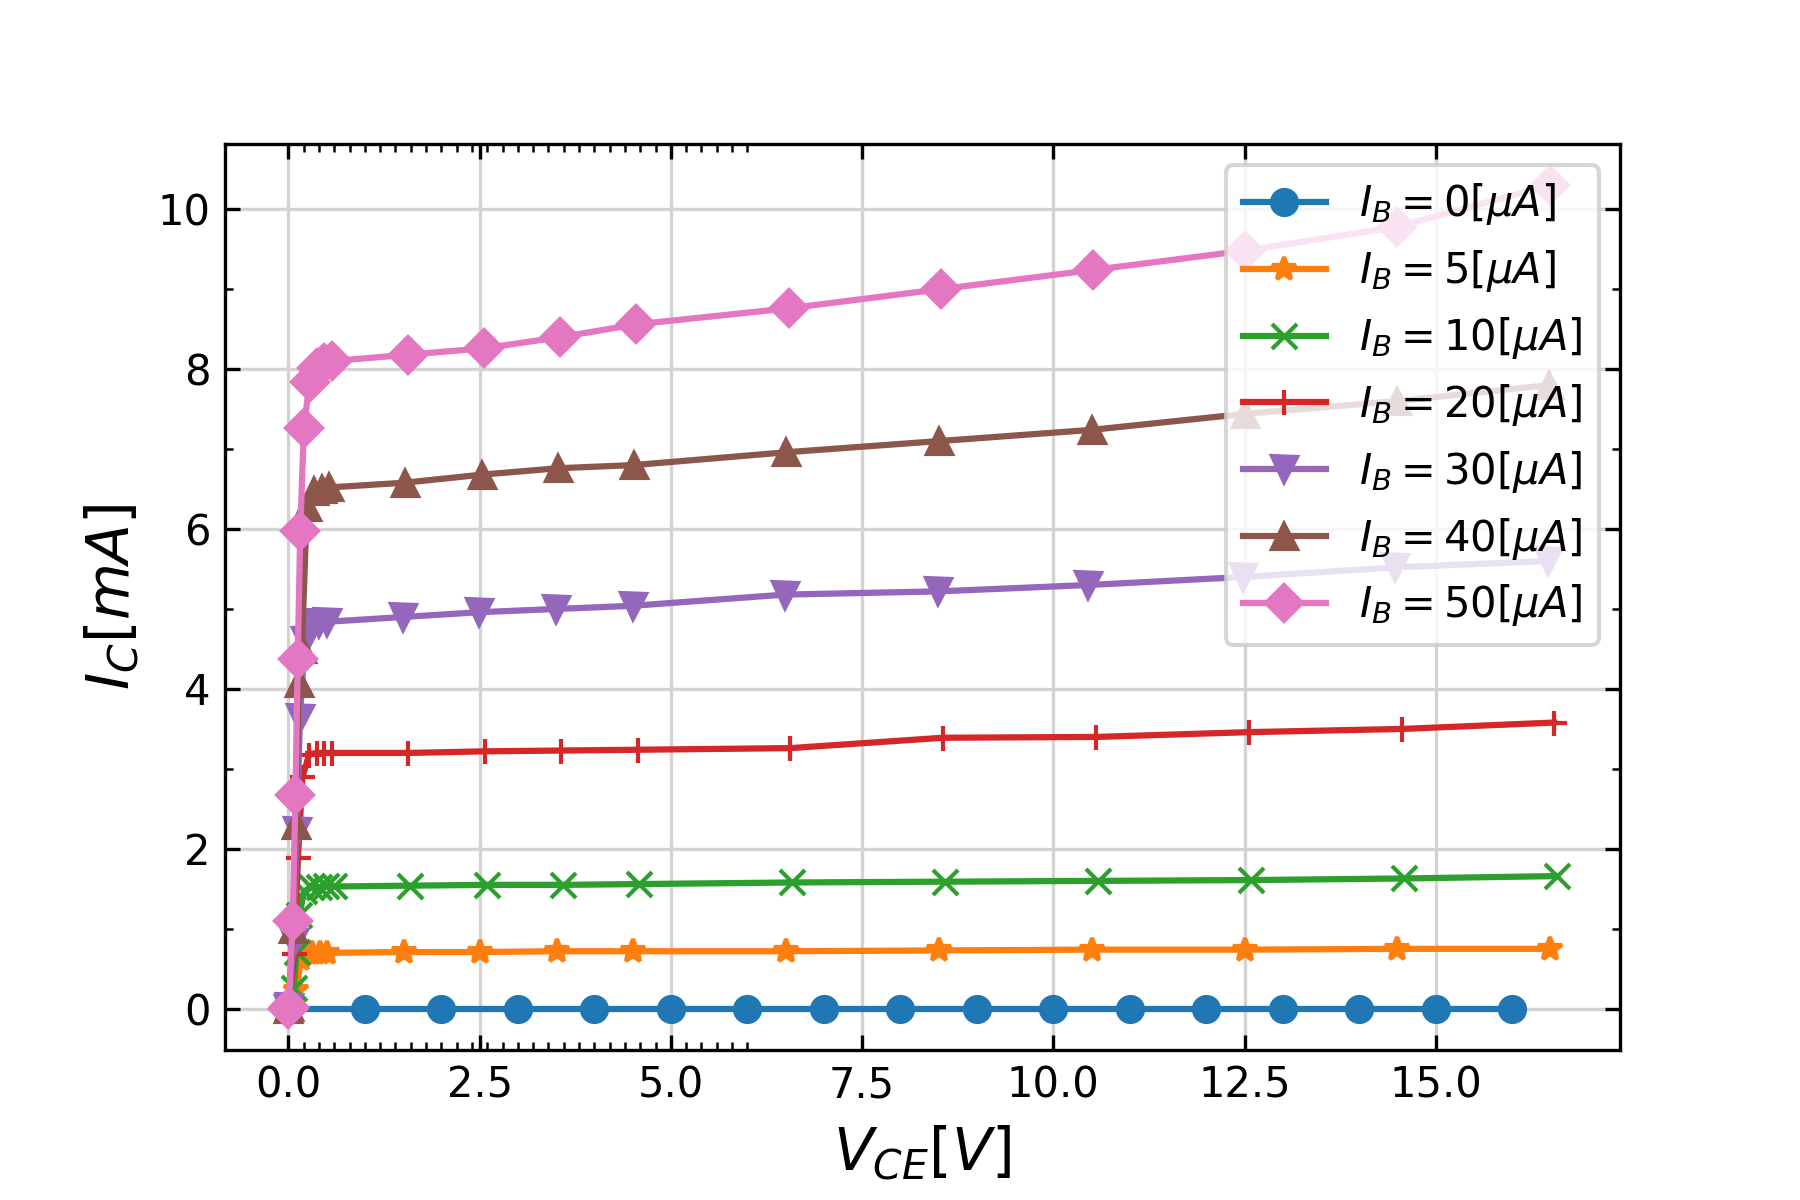
\includegraphics[height=55mm]{Ib-Vbe.png}
                      \caption{$I_B$-$V_{BE}$特性}
                    \end{minipage}
                \end{figure}
        \item 前述の周波数条件より発振周波数を求める.\\
                \begin{equation*}
                    f = \frac{1}{2\pi\sqrt{6}CR}
                \end{equation*}
                より,
                \begin{eqnarray*}
                    f & = & \frac{1}{2\pi\sqrt{6}CR}\\
                    & = & \frac{1}{2\pi\sqrt{6} \times 0.068 \times 10^-6 \times 1 \times 10^3}\\
                    & \simeq & 9.556 \times 10^-10\\
                \end{eqnarray*}
        \item 発信振幅を決める.(コレクタ側で振幅を$e_m$とする)\\
                
        \item 交流負荷$Z_{AC} \simeq B/D$を求める.(前述の周波数条件より$k = 6$なので$|Z_{AC}| \simeq 0.87R$)\\
                \begin{eqnarray*}
                    Z_{AC} & \simeq & B/D \\
                    & \simeq & 0.87 \times R \\
                    & \simeq & 0.87 \times 1 \times 10^3 \\
                    & \simeq & 870
                \end{eqnarray*}
        \item 動作点$Q$を交流負荷に対して直線部分の中央に決める.\\
              $V_{CEQ} \simeq e_m$,$I_{CQ} \simeq e_m/|Z_{AC}|$ \\
        \item 静特性曲線より$V_{BEQ}$,$I_{BQ}$を求める.
        \item 電源電圧を決める.$R_E$が決まる.
        \item 安定度(または,$f = I_2/I_{BQ}$)を決めて,$R_{B1}$,$R_{B2}$を求める.
      \end{enumerate}
      実際に作成した回路の実態配線図を以下に示す.
      \begin{figure}[H]
        \centering
        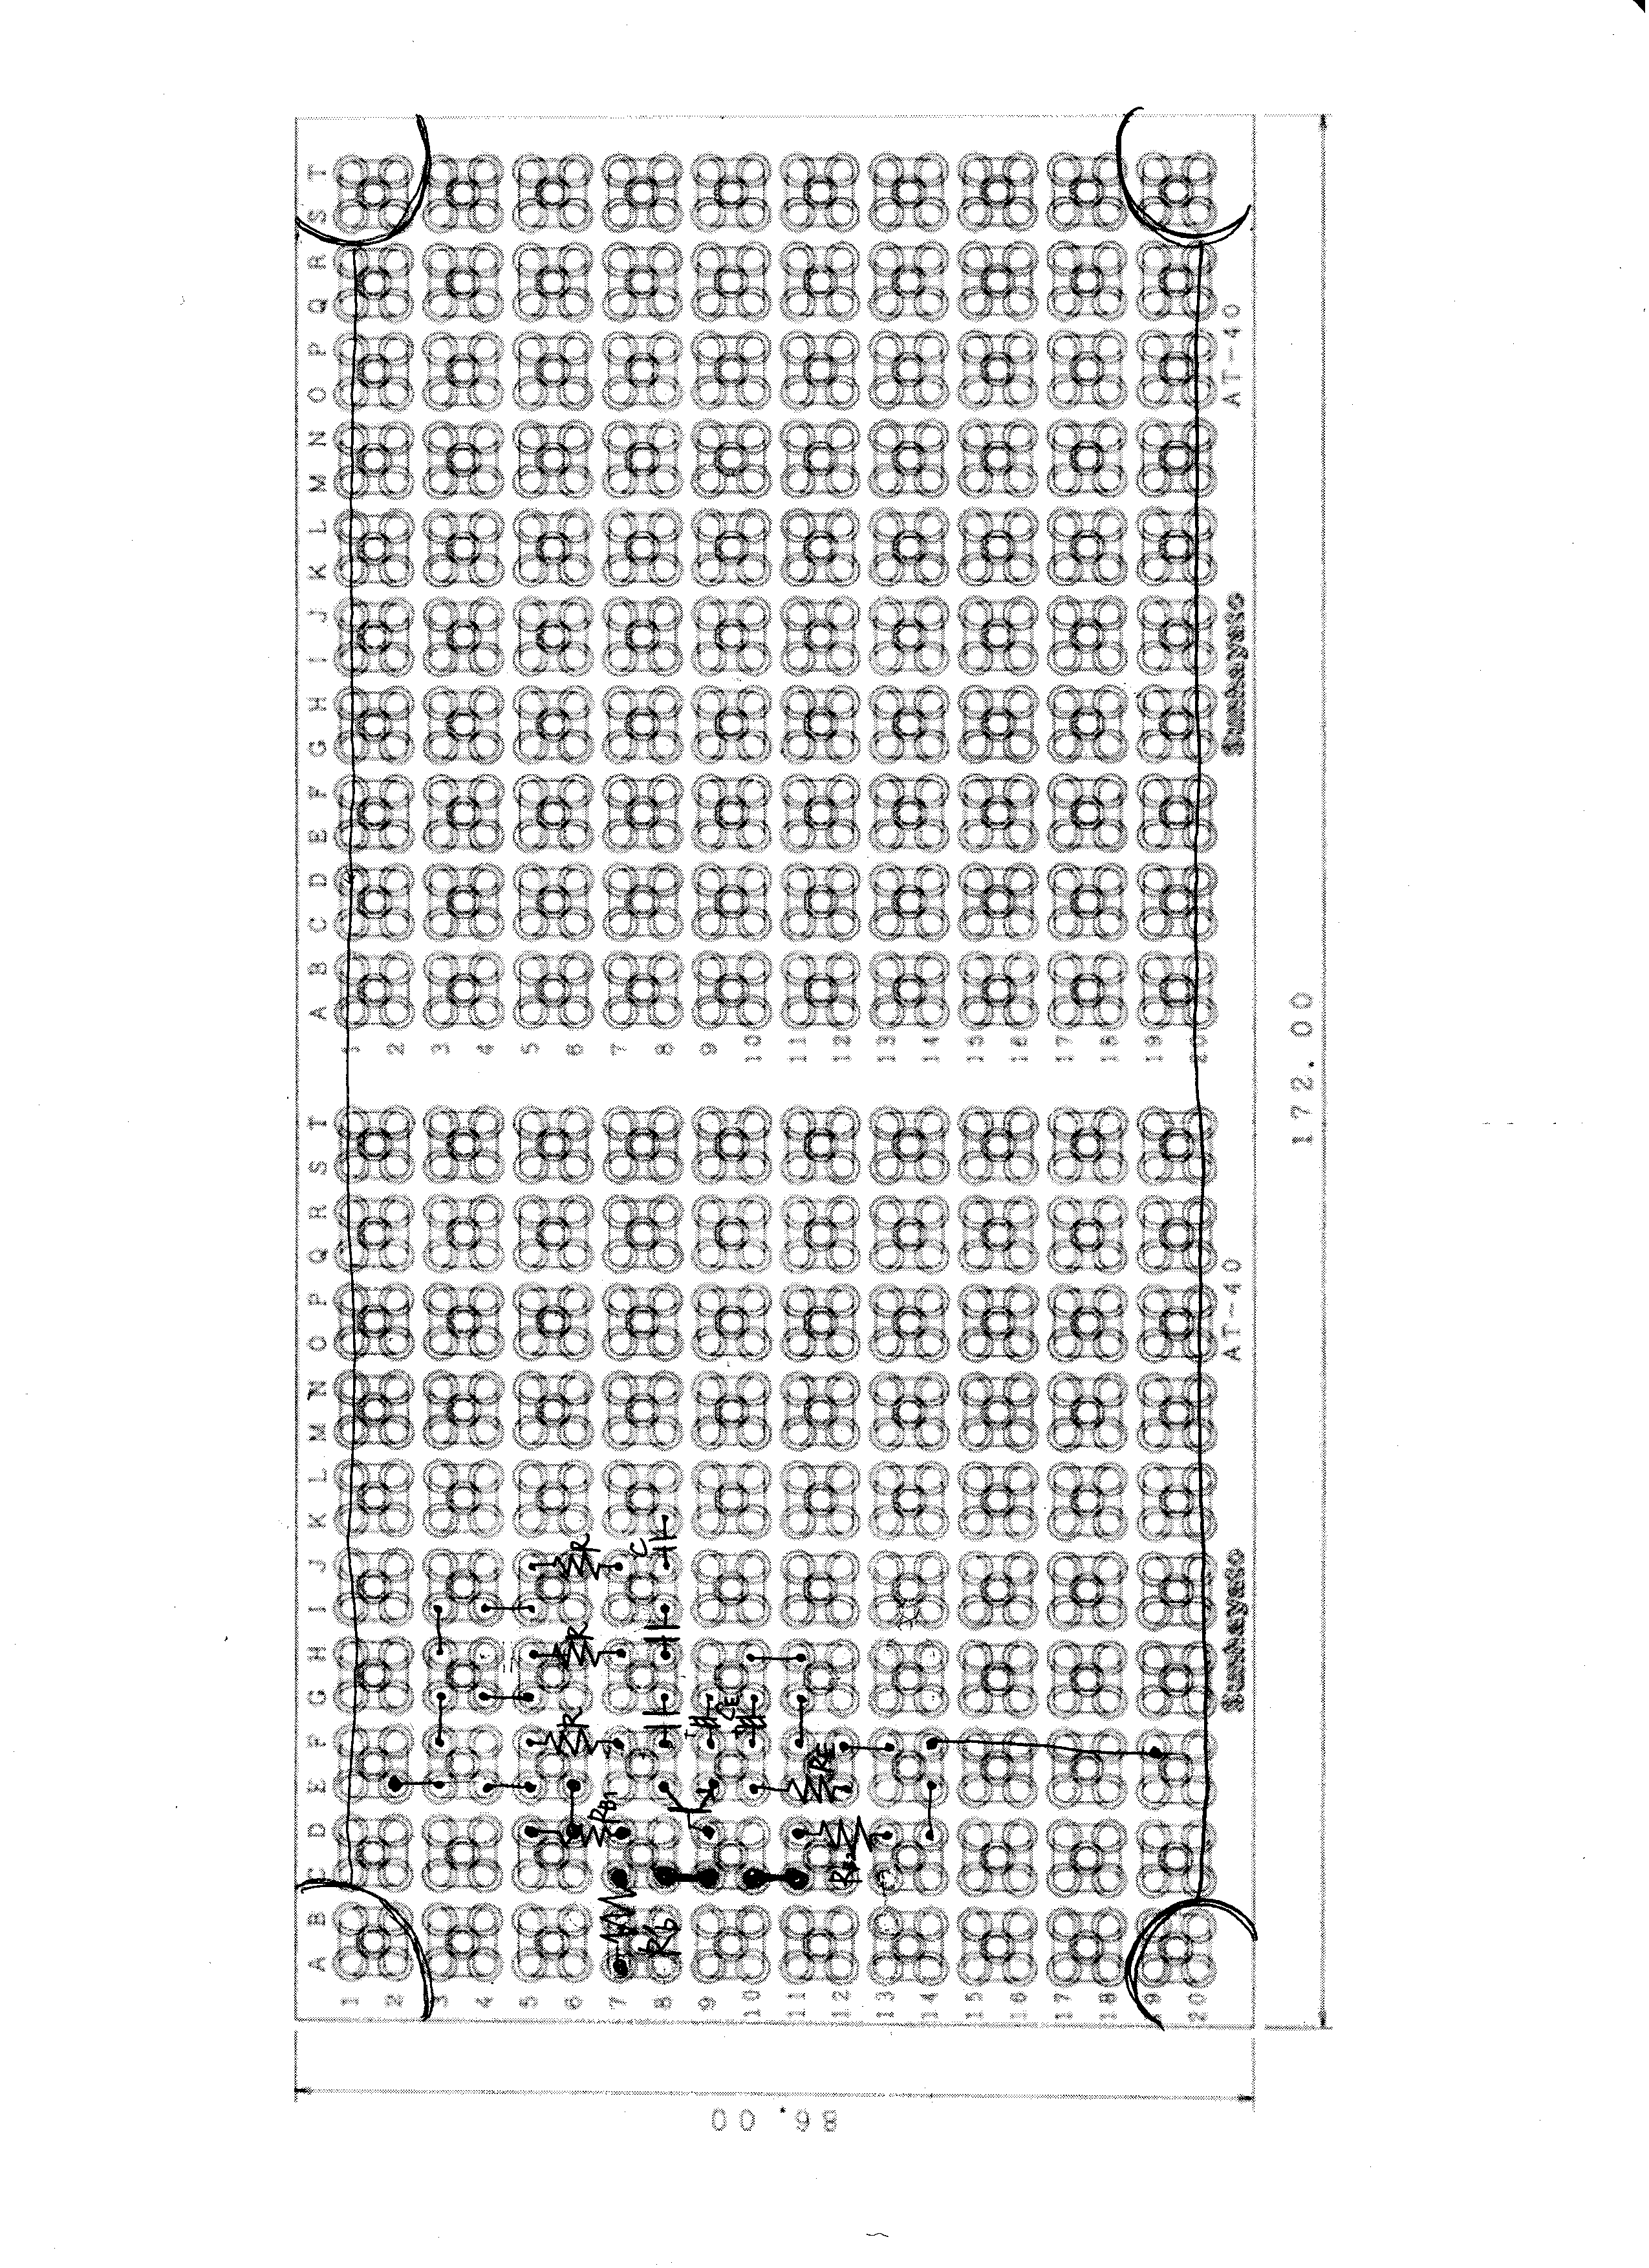
\includegraphics[width=75mm, angle=-90]{circuit.png}
        \figcaption{実態配線図}
      \end{figure}

    \subsection{CR移相回路のボード線図の測定}
    測定の結果を以下表\ref{tbl:1}に,グラフを図\ref{fig:ex-1}に示す.
        \small
        \begin{figure}[H]
            \centering
            \tblcaption{CR移相回路のボード線図}
            \label{tbl:1}
            % Please add the following required packages to your document preamble:
            % \usepackage{multirow}
            \begin{tabular}{|l|l|l|l|l|l|l|l|l|l|l|}
            \hline
            \multirow{3}{*}{f{[}kHz{]}} & \multirow{3}{*}{周期 T{[}s{]}} & \multirow{3}{*}{ei{[}V{]}} & \multirow{3}{*}{Ii{[}A{]}} & \multirow{3}{*}{-eo{[}V{]}} & \multirow{3}{*}{Io{[}A{]}} & \multicolumn{3}{l|}{位相差}             &          &          \\ \cline{7-11} 
                                        &                              &                            &                            &                             &                            & \multicolumn{3}{l|}{$\delta$t}              & 位相差      & 帰還率β     \\ \cline{7-11} 
                                        &                              &                            &                            &                             &                            & {[}sec{]} & θ{[}rad{]} & θ'{[}rad{]} & ∠Io/Ii   & |Ii/Io|  \\ \hline
            0.1                         & 1.00E-02                     & 3.68                       & 0.0184                     & 0.0352                      & 1.5.E-09                   & 3E-04     & 6E+00      & 1.8.E-01    & 4.53E+00 & 1.2.E+07 \\ \hline
            0.201                       & 4.98E-03                     & 3.64                       & 0.0182                     & 0.128                       & 1.1.E-08                   & 4E-04     & 6E+00      & 4.7.E-01    & 4.25E+00 & 1.7.E+06 \\ \hline
            0.504                       & 1.98E-03                     & 3.68                       & 0.0184                     & 0.688                       & 1.5.E-07                   & 3E-04     & 5E+00      & 9.5.E-01    & 3.76E+00 & 1.2.E+05 \\ \hline
            1.008                       & 9.92E-04                     & 3.88                       & 0.0194                     & 1.74                        & 7.5.E-07                   & 3E-04     & 5E+00      & 1.6.E+00    & 3.07E+00 & 2.6.E+04 \\ \hline
            2.007                       & 4.98E-04                     & 4.32                       & 0.0216                     & 3.08                        & 2.6.E-06                   & 2E-04     & 4E+00      & 2.3.E+00    & 2.44E+00 & 8.2.E+03 \\ \hline
            5.068                       & 1.97E-04                     & 4.88                       & 0.0244                     & 4.04                        & 8.7.E-06                   & 1E-04     & 3E+00      & 3.2.E+00    & 1.53E+00 & 2.8.E+03 \\ \hline
            10.072                      & 9.93E-05                     & 5.4                        & 0.027                      & 3.96                        & 1.7.E-05                   & 6E-05     & 3E+00      & 3.7.E+00    & 1.04E+00 & 1.6.E+03 \\ \hline
            20.132                      & 4.97E-05                     & 6.4                        & 0.032                      & 3.16                        & 2.7.E-05                   & 3E-05     & 2E+00      & 4.0.E+00    & 6.65E-01 & 1.2.E+03 \\ \hline
            50                          & 2.00E-05                     & 7.6                        & 0.038                      & 1.72                        & 3.7.E-05                   & 1E-05     & 2E+00      & 4.1.E+00    & 6.28E-01 & 1.0.E+03 \\ \hline
            100.18                      & 9.98E-06                     & 7.84                       & 0.0392                     & 0.944                       & 4.0.E-05                   & 7E-06     & 2E+00      & 4.4.E+00    & 3.06E-01 & 9.7.E+02 \\ \hline
            \end{tabular}
        \end{figure}
        \normalsize
        \begin{figure}[H]
            \centering
            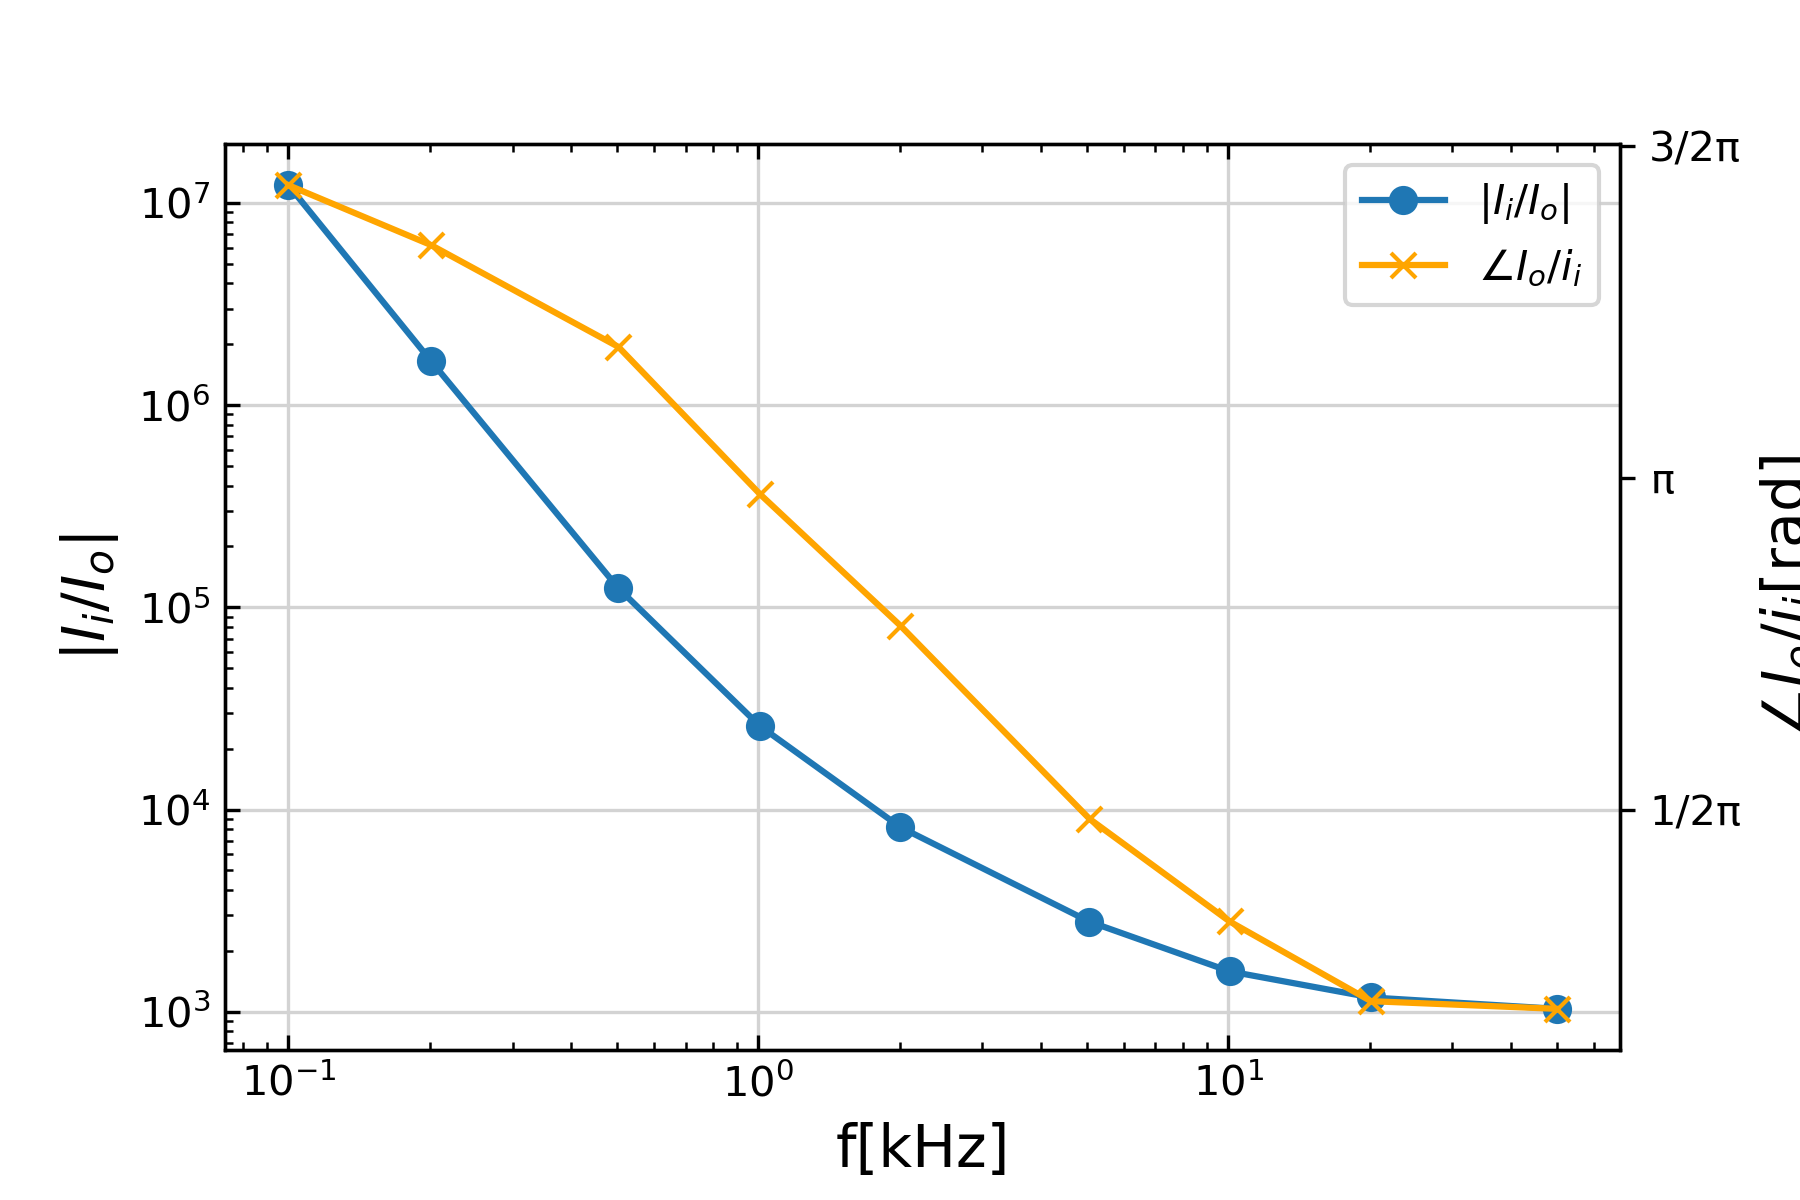
\includegraphics[width=\hsize]{ex_1.png}
            \figcaption{CR移相回路のボード線図}
            \label{fig:ex-1}
        \end{figure}

      \subsection{CR移相型発振回路の制作}
      以下図\ref{fig:ex-2}〜\ref{fig:ex-7}に測定した波形を示す.
      \begin{figure}[H]
        \centering
        \includegraphics[height=55mm]{104.bmp}
        \figcaption{}
        \label{fig:ex-2}
      \end{figure}
      \begin{figure}[H]
        \centering
        \includegraphics[height=55mm]{222.bmp}
        \figcaption{}
        \label{fig:ex-3}
      \end{figure}
      \begin{figure}[H]
        \centering
        \includegraphics[height=55mm]{472.bmp}
        \figcaption{}
        \label{fig:ex-4}
      \end{figure}
      \begin{figure}[H]
        \centering
        \includegraphics[height=55mm]{223.bmp}
        \figcaption{}
        \label{fig:ex-5}
      \end{figure}
      \begin{figure}[H]
        \centering
        \includegraphics[height=55mm]{683.bmp}
        \figcaption{}
        \label{fig:ex-6}
      \end{figure}
      \begin{figure}[H]
        \centering
        \includegraphics[height=55mm]{684.bmp}
        \figcaption{}
        \label{fig:ex-7}
      \end{figure}

      \subsection{移相器の容量-周波数特性の測定}
      以下,表\ref{tbl:2}に測定した値を,図\ref{fig:ex-8}にグラフを示す.
      \small
        \begin{figure}[H]
            \centering
            \tblcaption{容量-周波数特性}
            \label{tbl:2}
            % Please add the following required packages to your document preamble:
            % \usepackage{multirow}
            \begin{tabular}{|l|l|l|l|}
                \hline
                C{[}μF{]} & f{[}kHz{]} & epp{[}V{]} & 理論値f  \\ \hline
                0.0022    & 16.89      & 7.84       & 29.53 \\ \hline
                0.0047    & 8.197      & 8          & 13.82 \\ \hline
                0.022     & 2.016      & 8          & 2.95  \\ \hline
                0.068     & 0.6757     & 8          & 0.96  \\ \hline
                0.1       & 0.4545     & 8          & 0.65  \\ \hline
                0.68      & 0.07692    & 8          & 0.10  \\ \hline
                \end{tabular}
        \end{figure}
        \normalsize
        \begin{figure}[H]
            \centering
            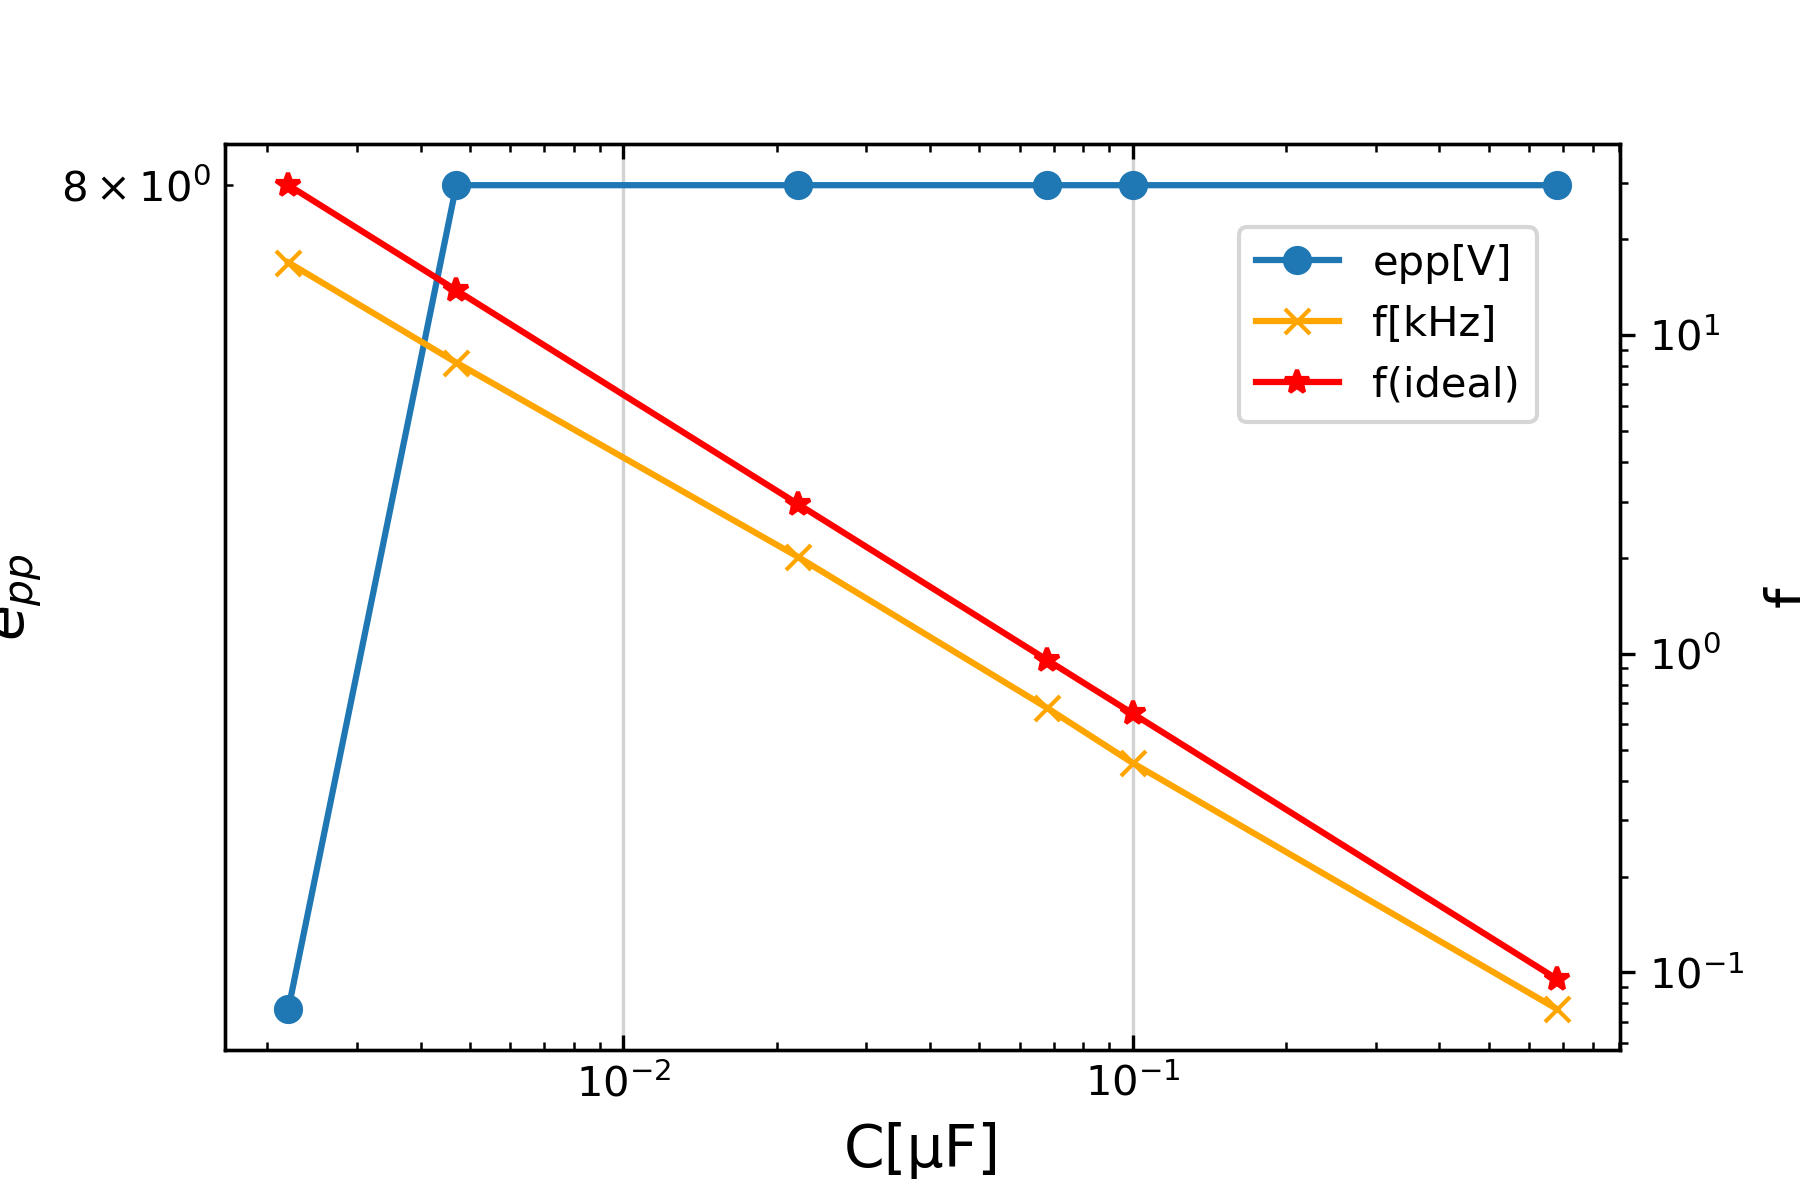
\includegraphics[width=\hsize]{ex_2.png}
            \figcaption{容量-周波数特性}
            \label{fig:ex-8}
          \end{figure}

      \section{吟味事項}
      \begin{enumerate}
          \item 発振周波数,基本はの発振振幅及び発振波形がどのようにして決まるか考察する.\\
                発振の最終的な振幅は,発振回路が安定な発振にはいるまでにどれくらい深く増幅回路の増幅特性の非線形領域に入り込むかによって決まると言える.
                つまり,発振は増幅回路の非線形性によって,安定な振幅に達するまで増大し続ける.この安定な動作状態は,回路の各部で自己矛盾のない形になっている.\\
                ~~いいかえれば,増幅回路の歪んだ出力が帰還回路を通って減衰されて増幅回路の入力となり,再び増幅されて出力側に現れたときもとの歪んだ出力と同じものになる.
                前回のトランジスタ増幅回路の入出力特性と,接続した移相回路の減衰特性(線形)を重ねて考え,その特性図を用いて具体的に発振の成長過程,安定な発振状態の点を示して説明する.\\
                ~~また,波形の歪みを少なくするためには,特性をどのように変化させればよいか,そのためには具体的に回路上でどの素子をどう変えればよいか説明する.\\
                さらに,発振振幅と発振波形の歪みとの関係を説明する.\\
                \\
                以下に前回の入出力特性を示す.
                \begin{figure}[H]
                    \centering
                    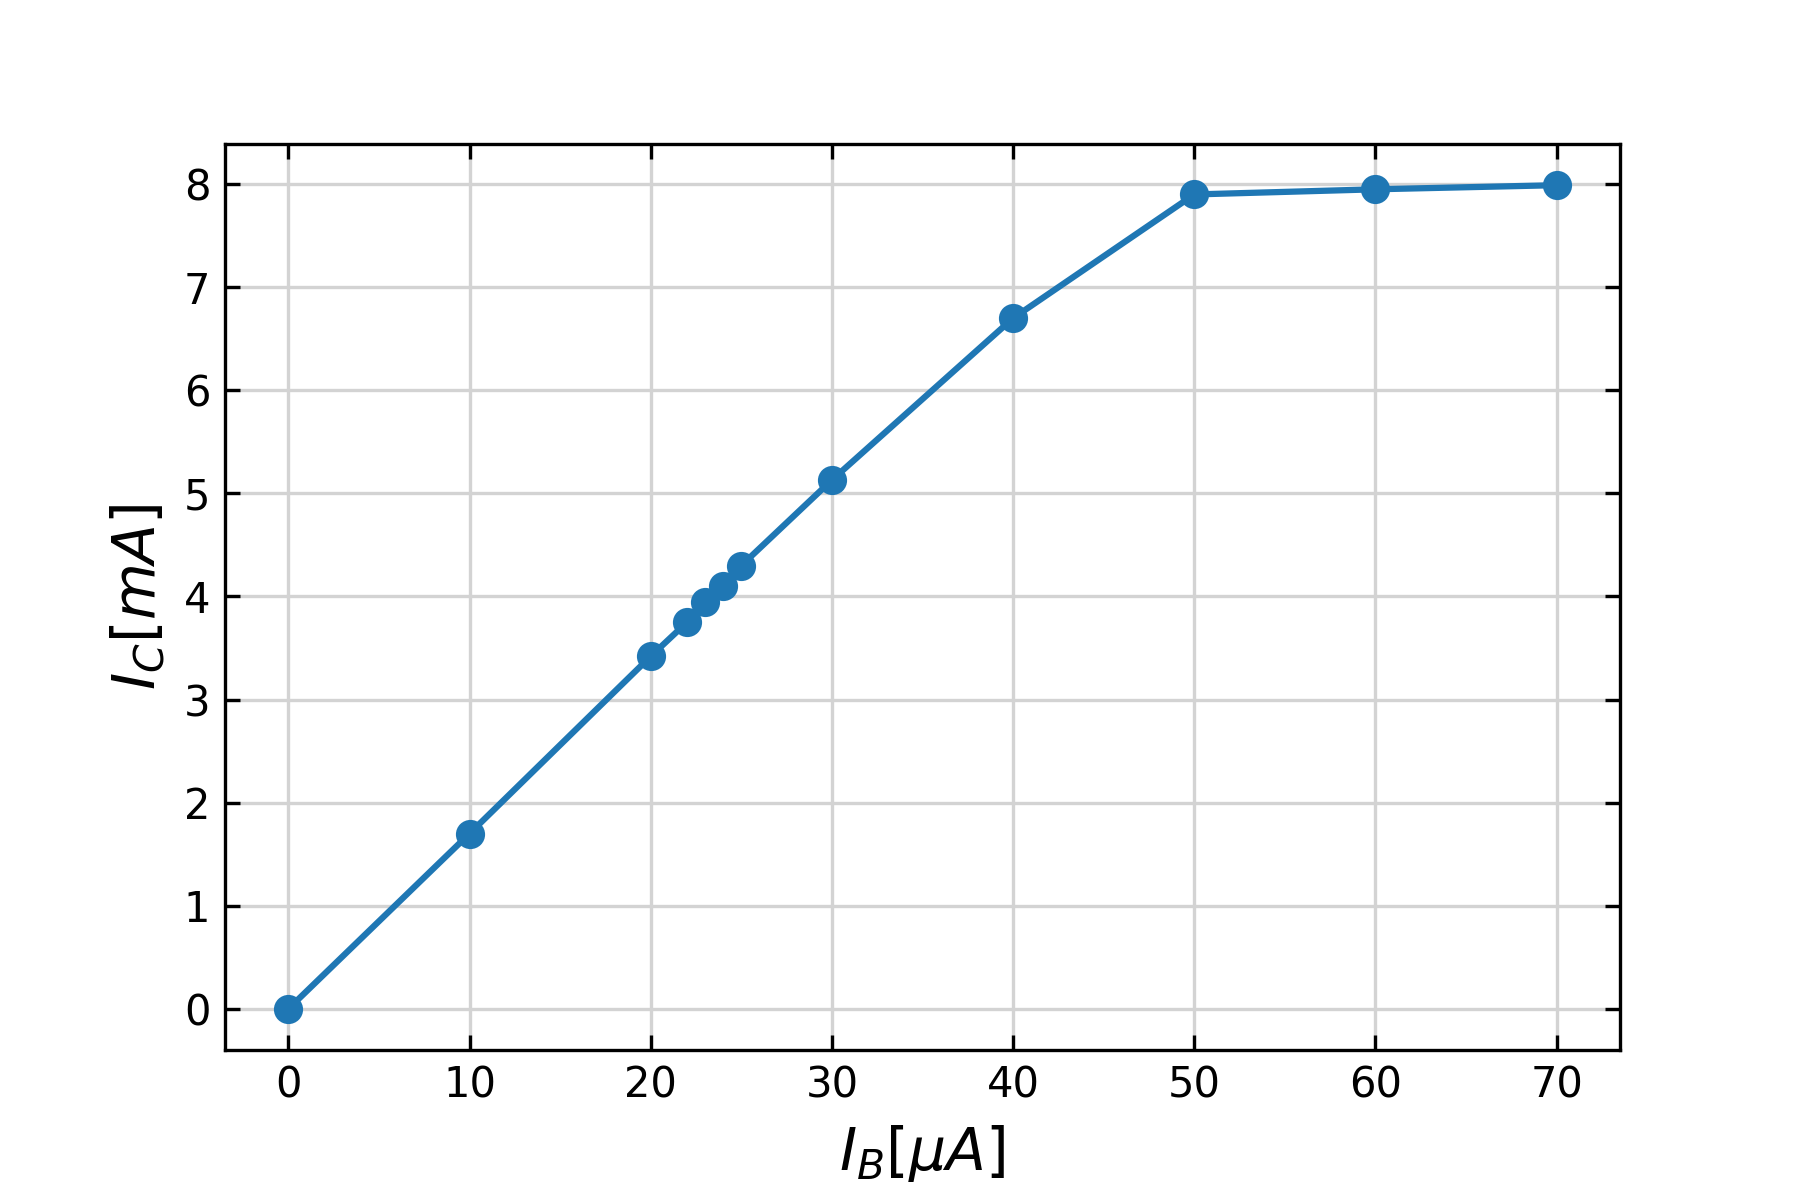
\includegraphics[width=\hsize]{ib-ic.png}
                    \figcaption{入出力特性}
                \end{figure}
                増幅と減衰を繰り返しながら一定の振幅を保つためには,入力の変化に比例して出力が変化する必要があると考えられるので,変化が少なくなる$I_B < 50[μA]$までの範囲で動作していると考えられる.
                また,波形の歪みを少なくするには,$I_B$の範囲をうまく調整してやれば良いので,回路の$R_b'$などを可変抵抗に変更するなどして,周波数に合わせて抵抗値を調節すればよいのではないかと予想する.

          \item 理論的に求めた発振周波数と実際に測定した発振周波数は同じであったか?違うと思うが,それは何故か考察する.理論式ではトランジスタの入力インピーダンス$r_{ie}$を$r_{ie} \simeq 0$とおいたが,増幅回路の入力インピーダンス$R_{ie}$があるとどうなるか考察する.\\

          理論値と測定値が違うのは,実際には0ではない$r_{ie}$を0とおいて計算を行ったためである.\\
          実際には,$r_{ie} \simeq 0$となるのは周波数が小さい時で有ることが,グラフの傾向からも観察できる.\\
      \end{enumerate}

\end{document}